\section{Hausdorff distance}
\nblink{brats/15a\_hausdorff\_distance.ipynb}

To calculate the similarity between two matrices, a distance function is required. The Hausdorff distance function is a special distance function,
which not only 

\begin{figure}[H]
\centering
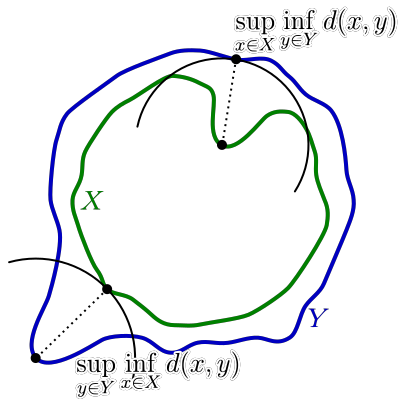
\includegraphics[width=8cm]{chapters/06_hdm/images/hausdorff_distance.png}
\caption{Visualization of the Hausdorff distance. The distance from set Y to set X is the maximal distance of a point on set Y to a point X \cite{hausdorffdistanceimage}}
\label{hausdorff_distance}
\end{figure}

\begin{figure}[H]
    \centering
    \begin{subfigure}{.5\textwidth}
        \centering
        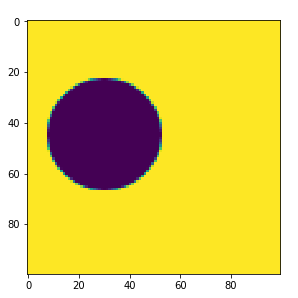
\includegraphics[width=.75\linewidth]{chapters/06_hdm/images/hdm_original.png}
        \caption{Original shape}
    \end{subfigure}%
    \begin{subfigure}{.5\textwidth}
        \centering
        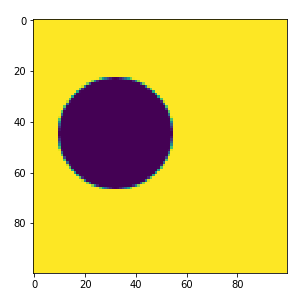
\includegraphics[width=.75\linewidth]{chapters/06_hdm/images/hdm_moved1.png}
        \caption{Shape moved slightly to the right}
    \end{subfigure}
    \caption{Hausdorff distance between the left and the right figure: 476. }
    \label{hdm_moved1}
\end{figure}


\begin{figure}[H]
    \centering
    \begin{subfigure}{.5\textwidth}
        \centering
        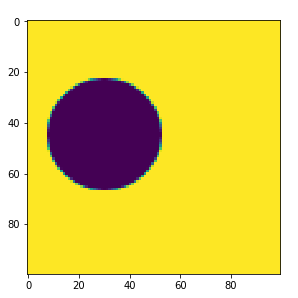
\includegraphics[width=.75\linewidth]{chapters/06_hdm/images/hdm_original.png}
        \caption{Original shape}
    \end{subfigure}%
    \begin{subfigure}{.5\textwidth}
        \centering
        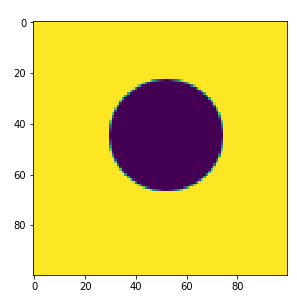
\includegraphics[width=.75\linewidth]{chapters/06_hdm/images/hdm_moved2.png}
        \caption{Shape moved to the right}
    \end{subfigure}
    \caption{Hausdorff distance between the left and the right figure: 1656. }
    \label{hdm_moved2}
\end{figure}

\begin{figure}[H]
    \centering
    \begin{subfigure}{.5\textwidth}
        \centering
        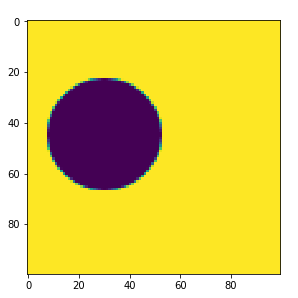
\includegraphics[width=.75\linewidth]{chapters/06_hdm/images/hdm_original.png}
        \caption{Original shape}
    \end{subfigure}%
    \begin{subfigure}{.5\textwidth}
        \centering
        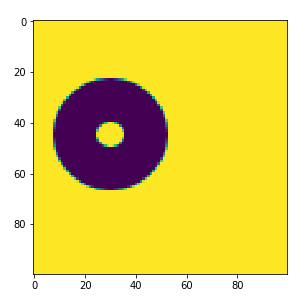
\includegraphics[width=.75\linewidth]{chapters/06_hdm/images/hdm_hole.png}
        \caption{Shape moved to the right}
    \end{subfigure}
    \caption{Hausdorff distance between the left and the right figure: 840. }
    \label{hdm_hole}
\end{figure}

\begin{figure}[H]
    \centering
    \begin{subfigure}{.5\textwidth}
        \centering
        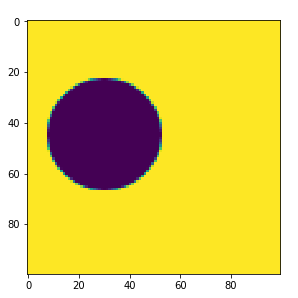
\includegraphics[width=.75\linewidth]{chapters/06_hdm/images/hdm_original.png}
        \caption{Original shape}
    \end{subfigure}%
    \begin{subfigure}{.5\textwidth}
        \centering
        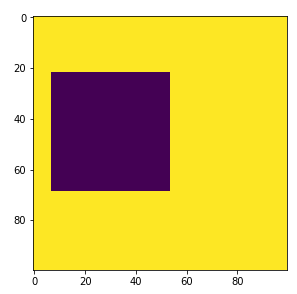
\includegraphics[width=.75\linewidth]{chapters/06_hdm/images/hdm_square.png}
        \caption{Shape moved to the right}
    \end{subfigure}
    \caption{Hausdorff distance between the left and the right figure: 1197. }
    \label{hdm_square}
\end{figure}


\begin{figure}[H]
    \centering
    \begin{subfigure}{.5\textwidth}
        \centering
        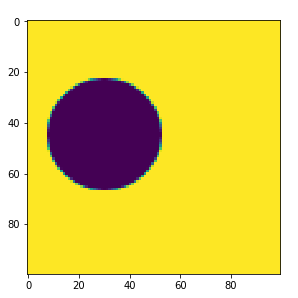
\includegraphics[width=.75\linewidth]{chapters/06_hdm/images/hdm_original.png}
        \caption{Original shape}
    \end{subfigure}%
    \begin{subfigure}{.5\textwidth}
        \centering
        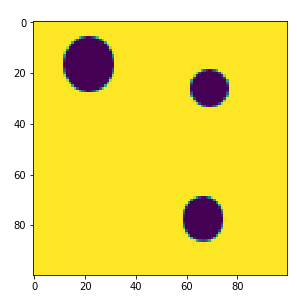
\includegraphics[width=.75\linewidth]{chapters/06_hdm/images/hdm_smaller_circles.png}
        \caption{Shape moved to the right}
    \end{subfigure}
    \caption{Hausdorff distance between the left and the right figure: 1353. }
    \label{hdm_smaller_circles}
\end{figure}
